% Options for packages loaded elsewhere
\PassOptionsToPackage{unicode}{hyperref}
\PassOptionsToPackage{hyphens}{url}
%
\documentclass[
  12pt,a4paper,lualatex,ja=standard]{bxjsarticle}
\usepackage{lmodern}
\usepackage{amsmath}
\usepackage{ifxetex,ifluatex}
\ifnum 0\ifxetex 1\fi\ifluatex 1\fi=0 % if pdftex
  \usepackage[T1]{fontenc}
  \usepackage[utf8]{inputenc}
  \usepackage{textcomp} % provide euro and other symbols
  \usepackage{amssymb}
\else % if luatex or xetex
  \usepackage{unicode-math}
  \defaultfontfeatures{Scale=MatchLowercase}
  \defaultfontfeatures[\rmfamily]{Ligatures=TeX,Scale=1}
\fi
% Use upquote if available, for straight quotes in verbatim environments
\IfFileExists{upquote.sty}{\usepackage{upquote}}{}
\IfFileExists{microtype.sty}{% use microtype if available
  \usepackage[]{microtype}
  \UseMicrotypeSet[protrusion]{basicmath} % disable protrusion for tt fonts
}{}
\makeatletter
\@ifundefined{KOMAClassName}{% if non-KOMA class
  \IfFileExists{parskip.sty}{%
    \usepackage{parskip}
  }{% else
    \setlength{\parindent}{0pt}
    \setlength{\parskip}{6pt plus 2pt minus 1pt}}
}{% if KOMA class
  \KOMAoptions{parskip=half}}
\makeatother
\usepackage{xcolor}
\IfFileExists{xurl.sty}{\usepackage{xurl}}{} % add URL line breaks if available
\IfFileExists{bookmark.sty}{\usepackage{bookmark}}{\usepackage{hyperref}}
\hypersetup{
  hidelinks,
  pdfcreator={LaTeX via pandoc}}
\urlstyle{same} % disable monospaced font for URLs
\usepackage{graphicx}
\makeatletter
\def\maxwidth{\ifdim\Gin@nat@width>\linewidth\linewidth\else\Gin@nat@width\fi}
\def\maxheight{\ifdim\Gin@nat@height>\textheight\textheight\else\Gin@nat@height\fi}
\makeatother
% Scale images if necessary, so that they will not overflow the page
% margins by default, and it is still possible to overwrite the defaults
% using explicit options in \includegraphics[width, height, ...]{}
\setkeys{Gin}{width=\maxwidth,height=\maxheight,keepaspectratio}
% Set default figure placement to htbp
\makeatletter
\def\fps@figure{htbp}
\makeatother
\setlength{\emergencystretch}{3em} % prevent overfull lines
\providecommand{\tightlist}{%
  \setlength{\itemsep}{0pt}\setlength{\parskip}{0pt}}
\setcounter{secnumdepth}{5}
\usepackage{indentfirst}
\parindent = 1em
\usepackage{dcolumn}
\newcolumntype{.}{D{.}{.}{-1}}
\usepackage{caption}
\captionsetup[table]{name=表}
\captionsetup[figure]{name=図}
\usepackage{hyperref}
\pagestyle{empty}
\usepackage{multicol}
\usepackage{ascmac}
\setpagelayout*{top=10truemm,bottom=30truemm,left=10truemm,right=10truemm}
\usepackage{tikz}
\usetikzlibrary{arrows.meta,decorations,decorations.pathreplacing,arrows,calc}
\usepackage{tabstackengine}
\usepackage{xcolor}
\usepackage{rotating}
\usepackage{txfonts}
\usepackage{fancybox}
\usepackage{dashbox}
\usepackage{tcolorbox}
\tcbuselibrary{theorems,skins}
\usepackage{siunitx}
\usepackage{framed}
\usepackage{enumerate}
\usepackage{lastpage}
\usepackage{pgfplots}
\pgfplotsset{compat=1.15}
\usepackage{mathrsfs}
\ifluatex
  \usepackage{selnolig}  % disable illegal ligatures
\fi

\author{}
\date{\vspace{-2.5em}}

\begin{document}

\renewcommand{\thefootnote}{}
\newcounter{kaunta}
\renewcommand{\thekaunta}{\arabic{kaunta}}
\newcommand{\kaunta}{\refstepcounter{kaunta}%
\thekaunta}
\def\question{\noindent\fbox{\large\makebox[1em]{\text{\kaunta}}} \hspace{1pt}}
\newcounter{skaunta}
\renewcommand{\theskaunta}{\arabic{skaunta}}
\newcommand{\skaunta}{\refstepcounter{skaunta}%
\theskaunta}
\def\squestion{(\text{\skaunta})\hspace{2.5pt}}
\newcommand{\maru}[1]{\raise0.2ex\hbox{\textcircled{\scriptsize{#1}}}}
\newcommand{\jsim}{\mathrel{\text{∽}}}
\newcommand{\jpara}{/\!/}
\newcounter{kurankaunta}
\renewcommand{\thekurankaunta}{\arabic{kurankaunta}}
\newcommand{\kurankaunta}{\refstepcounter{kurankaunta}%
\thekurankaunta}

\newcounter{kcounter}
\setcounter{kcounter}{0}
\newcommand{\kana}{\refstepcounter{kcounter}\ifthenelse{\value{kcounter}=1}{ア}{\ifthenelse{\value{kcounter}=2}{イ}{\ifthenelse{\value{kcounter}=3}{ウ}{\ifthenelse{\value{kcounter}=4}{エ}{\ifthenelse{\value{kcounter}=5}{オ} {\ifthenelse{\value{kcounter}=6}{カ}{\ifthenelse{\value{kcounter}=7}{キ}{\ifthenelse{\value{kcounter}=8}{ク}{\ifthenelse{\value{kcounter}=9}{ケ}{\ifthenelse{\value{kcounter}=10}{コ}{\ifthenelse{\value{kcounter}=11}{サ}{\ifthenelse{\value{kcounter}=12}{シ}{\ifthenelse{\value{kcounter}=13}{ス}{\ifthenelse{\value{kcounter}=14}{セ}{\ifthenelse{\value{kcounter}=15}{ソ}{\ifthenelse{\value{kcounter}=16}{タ}{\ifthenelse{\value{kcounter}=17}{チ}{\ifthenelse{\value{kcounter}=18}{ツ}{\ifthenelse{\value{kcounter}=19}{テ}{\ifthenelse{\value{kcounter}=20}{ト}{\ifthenelse{\value{kcounter}=21}{ナ}{\ifthenelse{\value{kcounter}=22}{ニ}{\ifthenelse{\value{kcounter}=23}{ヌ}{\ifthenelse{\value{kcounter}=24}{ネ}{\ifthenelse{\value{kcounter}=25}{ノ}{\ifthenelse{\value{kcounter}=26}{ハ}{\ifthenelse{\value{kcounter}=27}{ヒ}{\ifthenelse{\value{kcounter}=28}{フ}{\ifthenelse{\value{kcounter}=29}{ヘ}{\ifthenelse{\value{kcounter}=30}{ホ}{\ifthenelse{\value{kcounter}=31}{マ}{\ifthenelse{\value{kcounter}=32}{ミ}{\ifthenelse{\value{kcounter}=33}{ム}{\ifthenelse{\value{kcounter}=34}{メ}{\ifthenelse{\value{kcounter}=35}{モ}{\ifthenelse{\value{kcounter}=36}{ヤ}{\ifthenelse{\value{kcounter}=37}{ユ}{\ifthenelse{\value{kcounter}=38}{ヨ}{\ifthenelse{\value{kcounter}=39}{ラ}{\ifthenelse{\value{kcounter}=40}{リ}{\ifthenelse{\value{kcounter}=41}{ル}{\ifthenelse{\value{kcounter}=42}{レ}{\ifthenelse{\value{kcounter}=43}{ロ}{\ifthenelse{\value{kcounter}=44}{ワ}{・}}}}}}}}}}}}}}}}}}}}}}}}}}}}}}}}}}}}}}}}}}}}}

\newcommand{\kuran}[1]{\framebox[1.5cm][c]{\maru{\kana}}}
\newcommand{\sukuran}[1]{\framebox[1.5cm][c]{\maru{\kurankaunta}}}

\newcommand{\degre}{\ensuremath{^\circ}}

\newcommand{\myarc}[1]{
   \tikz [baseline = (N.base), every node/.style={}] {
      \node [inner sep = 0pt] (N) {$\mathrm{#1}$};
      \draw [line width = 0.4pt] plot [smooth, tension=1.3] coordinates {
         ($(N.north west) + (0.1ex,0)$)
         ($(N.north)      + (0,0.5ex)$)
         ($(N.north east) + (0,0)$)
      };
   }
}

\makeatletter
\newenvironment{figurehere}{\def\@captype{figure}}{}
\makeatother

\newcommand{\haiten}[1]{%
\begin{flushright}%
\footnotesize{<#1>}%
\end{flushright}%
}

\newcommand{\goku}[1]{\fbox{\phantom{\text{#1}} \quad}}

\newgeometry{top=10truemm,bottom=10truemm,left=20truemm,right=20truemm}

\thispagestyle{empty}
\begin{center}
\phantom{empty}

\vspace{60truemm}

\hspace{4em} {\HUGE\gtfamily\bfseries 数\hspace{2em}学}\hspace{1em}{\large \gtfamily \bfseries ($\mathbf{1}$年)}\\

\vspace{15truemm}

\hspace{2.5em}{\large \gtfamily \bfseries (この問題は定規とコンパスが必要です。)}

\vspace{64truemm}

{\large\gtfamily\bfseries 注\hspace{5em}意}

\end{center}

\centering
\begin{framed}
\begin{flushleft}
\begin{enumerate}[\Large \gtfamily 1]
  \item {\large 「開始」の合図があるまでは,開いてはいけません。}

  \item {\large 問題は\pageref{LastPage}ページまであります。}

  \item {\large 「開始」の合図があったら,まず,問題用紙・解答用紙に,組・番号と名前などを書きなさい。}

  \item {\large 答えは,すべて解答用紙に書きなさい。また、所定の欄に濃くはっきりと書きなさい。}

  \item {\large 「終了」の合図で,すぐ鉛筆をおき,解答用紙を裏返しにしなさい。}
\end{enumerate}
\end{flushleft}
\end{framed}

\vspace{14mm}

\begin{center}
{\large \underline{\hspace{30mm}組 \hspace{30mm}番 \hspace{15mm} 名前 \hspace{60mm}}}
\end{center}

\newpage

  \href{空白ページのための全角スペースあり。}{} \newpage

\pagestyle{plain}
\pagenumbering{arabic}

\begin{flushleft}

\noindent\fbox{\large\makebox[1em]{\text{\refstepcounter{kaunta}%
\arabic{kaunta}}}} \hspace{1pt}次の空欄に当てはまる適切な語句を選び、記号で答えなさい。

%
\begin{flushright}%
\footnotesize{<知・技$2 \times 12$点>}%
\end{flushright}%


各階級について、最初の階級からその階級までの度数を合計したものを\underline{(\text{\refstepcounter{skaunta}%
\arabic{skaunta}})\hspace{2.5pt}ア \, 累積度数 / イ \, 度数}という。

全体の度数が異なる異なるデータを比較するときには、度数の代わりに、度数の合計に対する割合を用いるとよい。この値を\underline{(\text{\refstepcounter{skaunta}%
\arabic{skaunta}})\hspace{2.5pt}ア \, 絶対度数 /  イ \, 相対度数}という。各階級について、最初の階級からその階級までの相対度数を合計したものを\underline{(\text{\refstepcounter{skaunta}%
\arabic{skaunta}})\hspace{2.5pt}ア \, 累積相対度数 / イ \, 堆積相対度数}という。

度数分布表から、度数や相対度数を柱状に整理した図を\underline{(\text{\refstepcounter{skaunta}%
\arabic{skaunta}})\hspace{2.5pt}ア \, ヒストグラム / イ \, ピストグラム}といい、おのおの長方形の上の辺の中点を結んだ折れ線を\underline{(\text{\refstepcounter{skaunta}%
\arabic{skaunta}})\hspace{2.5pt}ア \, 折れ線グラフ / イ \, 度数折れ線 }という。

データの分布の特徴を調べたり伝えたりするときにデータの代表的な値を用いることがある。このような値を\underline{(\text{\refstepcounter{skaunta}%
\arabic{skaunta}})\hspace{2.5pt}ア \, 代表値 / イ \, 絶対値}という。

個々のデータの値の合計をデータの総数でわった値を\underline{(\text{\refstepcounter{skaunta}%
\arabic{skaunta}})\hspace{2.5pt}ア \, 平均値 / イ \, 最小値}という。調べようとするデータの値を大きさの順に並べたときの中央の値を\underline{(\text{\refstepcounter{skaunta}%
\arabic{skaunta}})\hspace{2.5pt}ア \, 中央値 / イ \, 中心値}という。また、データの中でもっとも多く出てくる値を\underline{(\text{\refstepcounter{skaunta}%
\arabic{skaunta}})\hspace{2.5pt}ア \, 最瀕値 / イ \, 最大値}という。度数分布表では、度数のもっとも多い階級の階級値を用いる。データの散らばりぐらいを表す数値として、最大値から最小値をひいた値を用いることがある。このような値を分布の\underline{(\text{\refstepcounter{skaunta}%
\arabic{skaunta}})\hspace{2.5pt}ア \, 範囲 / イ \, 幅}という。

結果が偶然に左右される実験や観察を行うとき、あることがらが起こると期待される程度を数で表したものを、そのことがらの起こる\underline{(\text{\refstepcounter{skaunta}%
\arabic{skaunta}})\hspace{2.5pt}ア \, 期待値 / イ \, 確率}という。確率が$p$であるということは同じ実験や観察を多数回くり返すとき、そのことがらの起こる\underline{(\text{\refstepcounter{skaunta}%
\arabic{skaunta}})\hspace{2.5pt}ア \, 回数 / イ \, 相対度数}が$p$に限りなく近づくという意味をもつ。

\newpage

\setcounter{skaunta}{0}

\noindent\fbox{\large\makebox[1em]{\text{\refstepcounter{kaunta}%
\arabic{kaunta}}}} \hspace{1pt}次の$\raise 0.2ex\hbox{\textcircled{\scriptsize{ア}}} \sim \raise 0.2ex\hbox{\textcircled{\scriptsize{オ}}}$のなかから、それらをふくむ平面が1つに決まるものをすべて選び、記号で答えなさい。

%
\begin{flushright}%
\footnotesize{<知・技$2$点>}%
\end{flushright}%


\begin{multicols}{2}
\begin{itemize}
\item[\raise 0.2ex\hbox{\textcircled{\scriptsize{ア}}}] 1つの直線上にある3点
\item[\raise 0.2ex\hbox{\textcircled{\scriptsize{イ}}}] 1つの直線上にない3点
\item[\raise 0.2ex\hbox{\textcircled{\scriptsize{ウ}}}] 1つの直線とその上にない1点
\item[\raise 0.2ex\hbox{\textcircled{\scriptsize{エ}}}] 交わる2つの直線
\item[\raise 0.2ex\hbox{\textcircled{\scriptsize{オ}}}] 平行な2つの直線
\end{itemize}
\end{multicols}

\vspace{7mm}

\begin{multicols}{2}

\noindent\fbox{\large\makebox[1em]{\text{\refstepcounter{kaunta}%
\arabic{kaunta}}}} \hspace{1pt}右の図の三角柱について、次の問に答えなさい。ただし、$\triangle$ABCは直角二等辺三角形である。

%
\begin{flushright}%
\footnotesize{<知・技$2 \times 7$点>}%
\end{flushright}%


(\text{\refstepcounter{skaunta}%
\arabic{skaunta}})\hspace{2.5pt}辺ABと平行な辺を答えなさい。

\vspace{3mm}\null

\columnbreak

\begin{center}
\def\@captype{figure}
\includegraphics[height=35mm]{img/img1.jpg}

\end{center}

\end{multicols}

(\text{\refstepcounter{skaunta}%
\arabic{skaunta}})\hspace{2.5pt}辺ABとねじれの位置にある辺をすべて答えなさい。

\vspace{10mm}

(\text{\refstepcounter{skaunta}%
\arabic{skaunta}})\hspace{2.5pt}面ABCと垂直な辺をすべて答えなさい。

\vspace{10mm}

(\text{\refstepcounter{skaunta}%
\arabic{skaunta}})\hspace{2.5pt}辺DEと垂直な面を答えなさい。

\vspace{10mm}

(\text{\refstepcounter{skaunta}%
\arabic{skaunta}})\hspace{2.5pt}面DEFと垂直な面をすべて答えなさい。

\vspace{10mm}

(\text{\refstepcounter{skaunta}%
\arabic{skaunta}})\hspace{2.5pt}面BEFCと垂直な面をすべて答えなさい。

\vspace{10mm}

(\text{\refstepcounter{skaunta}%
\arabic{skaunta}})\hspace{2.5pt}面ADFCと面ADEBのつくる角は何度ですか。

\vspace{10mm}

\newpage

\setcounter{skaunta}{0}

\begin{multicols}{2}

\noindent\fbox{\large\makebox[1em]{\text{\refstepcounter{kaunta}%
\arabic{kaunta}}}} \hspace{1pt}右の図のような底面の1辺が2cmで、側面の二等辺三角形の等しい辺が3cmである正三角錐の展開図を、側面をつないでかきなさい。\textbf{この問に限り}、定規を使って長さを測ってもかまいません。

%
\begin{flushright}%
\footnotesize{<知・技2点>}%
\end{flushright}%


\columnbreak

\begin{center}
\def\@captype{figure}
\includegraphics[height=30mm]{img/img2.jpg}

\end{center}

\end{multicols}

\vfill

\setcounter{skaunta}{0}
\noindent\fbox{\large\makebox[1em]{\text{\refstepcounter{kaunta}%
\arabic{kaunta}}}} \hspace{1pt}次の(1)$\sim$(4)の投影図は、直方体、三角錐、四角錐、円柱、円錐、球のうち、どの立体を表していますか。

%
\begin{flushright}%
\footnotesize{<知・技$2 \times 4$点>}%
\end{flushright}%


\begin{multicols}{2}
(\text{\refstepcounter{skaunta}%
\arabic{skaunta}})\hspace{2.5pt}

\begin{center}
\def\@captype{figure}
\includegraphics[height=35mm]{img/img3.jpg}

\end{center}

\columnbreak

(\text{\refstepcounter{skaunta}%
\arabic{skaunta}})\hspace{2.5pt}

\begin{center}
\def\@captype{figure}
\includegraphics[height=35mm]{img/img4.jpg}

\end{center}

\end{multicols}

\vfill

\begin{multicols}{2}
(\text{\refstepcounter{skaunta}%
\arabic{skaunta}})\hspace{2.5pt}

\begin{center}
\def\@captype{figure}
\includegraphics[height=35mm]{img/img5.jpg}

\end{center}

\columnbreak

(\text{\refstepcounter{skaunta}%
\arabic{skaunta}})\hspace{2.5pt}

\begin{center}
\def\@captype{figure}
\includegraphics[height=35mm]{img/img6.jpg}

\end{center}

\end{multicols}

\vfill
\newpage

\setcounter{skaunta}{0}
\noindent\fbox{\large\makebox[1em]{\text{\refstepcounter{kaunta}%
\arabic{kaunta}}}} \hspace{1pt}次の立体の体積を求めなさい。

%
\begin{flushright}%
\footnotesize{<知・技$2 \times 6$点>}%
\end{flushright}%


\begin{multicols}{3}

(\text{\refstepcounter{skaunta}%
\arabic{skaunta}})\hspace{2.5pt}

\begin{center}
\def\@captype{figure}
\includegraphics[height=30mm]{img/img7.jpg}

\end{center}

\columnbreak

(\text{\refstepcounter{skaunta}%
\arabic{skaunta}})\hspace{2.5pt}

\begin{center}
\def\@captype{figure}
\includegraphics[height=30mm]{img/img8.jpg}

\end{center}

\columnbreak

(\text{\refstepcounter{skaunta}%
\arabic{skaunta}})\hspace{2.5pt}

\begin{center}
\def\@captype{figure}
\includegraphics[height=30mm]{img/img9.jpg}

\end{center}

\end{multicols}

\vfill

\begin{multicols}{3}

(\text{\refstepcounter{skaunta}%
\arabic{skaunta}})\hspace{2.5pt}

\begin{center}
\def\@captype{figure}
\includegraphics[height=30mm]{img/img10.jpg}

\end{center}

\columnbreak

(\text{\refstepcounter{skaunta}%
\arabic{skaunta}})\hspace{2.5pt}

\begin{center}
\def\@captype{figure}
\includegraphics[height=30mm]{img/img14.jpg}

\end{center}

\columnbreak

(\text{\refstepcounter{skaunta}%
\arabic{skaunta}})\hspace{2.5pt}

\begin{center}
\def\@captype{figure}
\includegraphics[height=30mm]{img/img12.jpg}

\end{center}

\end{multicols}

\vfill

\setcounter{skaunta}{0}
\noindent\fbox{\large\makebox[1em]{\text{\refstepcounter{kaunta}%
\arabic{kaunta}}}} \hspace{1pt}次の立体の表面積を求めなさい。

%
\begin{flushright}%
\footnotesize{<知・技$2 \times 3$点>}%
\end{flushright}%


\begin{multicols}{3}

(\text{\refstepcounter{skaunta}%
\arabic{skaunta}})\hspace{2.5pt}

\begin{center}
\def\@captype{figure}
\includegraphics[height=30mm]{img/img13.jpg}

\end{center}

\columnbreak

(\text{\refstepcounter{skaunta}%
\arabic{skaunta}})\hspace{2.5pt}

\begin{center}
\def\@captype{figure}
\includegraphics[height=30mm]{img/img11.jpg}

\end{center}

\columnbreak

(\text{\refstepcounter{skaunta}%
\arabic{skaunta}})\hspace{2.5pt}

\begin{center}
\def\@captype{figure}
\includegraphics[height=30mm]{img/img12.jpg}

\end{center}

\end{multicols}

\vfill

\newpage

\setcounter{skaunta}{0}

\noindent\fbox{\large\makebox[1em]{\text{\refstepcounter{kaunta}%
\arabic{kaunta}}}} \hspace{1pt}次の資料はあるクラスの生徒10人の数学のテストの点数を表している。

%
\begin{flushright}%
\footnotesize{<知・技$2 \times 4$点>}%
\end{flushright}%


\begin{center}
\begin{tabular}{|cccccccccc|}
\hline
76 & 63 & 84 & 59 & 70 & 84 & 91 & 64 & 82 & 84 \\
\hline
\end{tabular}
\end{center}

\begin{multicols}{2}

(\text{\refstepcounter{skaunta}%
\arabic{skaunta}})\hspace{2.5pt}平均値を求めなさい。

\columnbreak

(\text{\refstepcounter{skaunta}%
\arabic{skaunta}})\hspace{2.5pt}中央値を求めなさい。

\end{multicols}

\vspace{3mm}

\begin{multicols}{2}

(\text{\refstepcounter{skaunta}%
\arabic{skaunta}})\hspace{2.5pt}最瀕値を求めなさい。

\columnbreak

(\text{\refstepcounter{skaunta}%
\arabic{skaunta}})\hspace{2.5pt}範囲を求めなさい。

\end{multicols}

\vspace{3mm}

\begin{multicols}{2}

\setcounter{skaunta}{0}
\noindent\fbox{\large\makebox[1em]{\text{\refstepcounter{kaunta}%
\arabic{kaunta}}}} \hspace{1pt}さやかさんたちは,A中学校とB中学校のどちらのほうが通学時間が長い傾向にあるかを話し合っている。右の表は,A中学校の生徒35人とB中学校の生徒50人の片道の通学時間を,度数分布表に整理したものである。

%
\begin{flushright}%
\footnotesize{<知・技(1)(5)(7)2点、(4)6点、\\思・判・表(2)(3)(6)3点>}%
\end{flushright}%


【$\mathbf{I}$】次の会話を読んで問に答えなさい。

\columnbreak

\begin{tabular}{|c|c|c|}
\hline
階級(分) & A中学校(人) & B中学校(人)\\
\hline
\footnotesize{以上}\phantom{$\sim$} \footnotesize{未満} & & \\
$0 \sim 10$  & 3 & 6 \\
$10 \sim 20$ & 5 & 9 \\
$20 \sim 30$ & 6 & 11 \\
$30 \sim 40$ & 11 & 12 \\
$40 \sim 50$ & 6 & 7 \\
$50 \sim 60$ & 4 & 5 \\
\hline
合計 & 35 & 50 \\
\hline

\end{tabular}

\end{multicols}

\begin{screen}
\begin{itemize}
\setlength{\itemindent}{1em}
\item[さやか:]度数分布表からどんなことがわかるのかな。
\item[たくま:]この度数分布表の階級の幅は\framebox[1.5cm][c]{\raise 0.2ex\hbox{\textcircled{\scriptsize{\refstepcounter{kcounter}\ifthenelse{\value{kcounter}=1}{ア}{\ifthenelse{\value{kcounter}=2}{イ}{\ifthenelse{\value{kcounter}=3}{ウ}{\ifthenelse{\value{kcounter}=4}{エ}{\ifthenelse{\value{kcounter}=5}{オ} {\ifthenelse{\value{kcounter}=6}{カ}{\ifthenelse{\value{kcounter}=7}{キ}{\ifthenelse{\value{kcounter}=8}{ク}{\ifthenelse{\value{kcounter}=9}{ケ}{\ifthenelse{\value{kcounter}=10}{コ}{\ifthenelse{\value{kcounter}=11}{サ}{\ifthenelse{\value{kcounter}=12}{シ}{\ifthenelse{\value{kcounter}=13}{ス}{\ifthenelse{\value{kcounter}=14}{セ}{\ifthenelse{\value{kcounter}=15}{ソ}{\ifthenelse{\value{kcounter}=16}{タ}{\ifthenelse{\value{kcounter}=17}{チ}{\ifthenelse{\value{kcounter}=18}{ツ}{\ifthenelse{\value{kcounter}=19}{テ}{\ifthenelse{\value{kcounter}=20}{ト}{\ifthenelse{\value{kcounter}=21}{ナ}{\ifthenelse{\value{kcounter}=22}{ニ}{\ifthenelse{\value{kcounter}=23}{ヌ}{\ifthenelse{\value{kcounter}=24}{ネ}{\ifthenelse{\value{kcounter}=25}{ノ}{\ifthenelse{\value{kcounter}=26}{ハ}{\ifthenelse{\value{kcounter}=27}{ヒ}{\ifthenelse{\value{kcounter}=28}{フ}{\ifthenelse{\value{kcounter}=29}{ヘ}{\ifthenelse{\value{kcounter}=30}{ホ}{\ifthenelse{\value{kcounter}=31}{マ}{\ifthenelse{\value{kcounter}=32}{ミ}{\ifthenelse{\value{kcounter}=33}{ム}{\ifthenelse{\value{kcounter}=34}{メ}{\ifthenelse{\value{kcounter}=35}{モ}{\ifthenelse{\value{kcounter}=36}{ヤ}{\ifthenelse{\value{kcounter}=37}{ユ}{\ifthenelse{\value{kcounter}=38}{ヨ}{\ifthenelse{\value{kcounter}=39}{ラ}{\ifthenelse{\value{kcounter}=40}{リ}{\ifthenelse{\value{kcounter}=41}{ル}{\ifthenelse{\value{kcounter}=42}{レ}{\ifthenelse{\value{kcounter}=43}{ロ}{\ifthenelse{\value{kcounter}=44}{ワ}{・}}}}}}}}}}}}}}}}}}}}}}}}}}}}}}}}}}}}}}}}}}}}}}}}分だね。
\item[なおき:]最大値や最小値はこの表からは読みとれないね。
\item[さやか:]表の値を見るだけだと違いがわかりにくいから,代表値を求めて比べてみよう。
\item[たくま:]最頻値はどちらの中学校も\framebox[1.5cm][c]{\raise 0.2ex\hbox{\textcircled{\scriptsize{\refstepcounter{kcounter}\ifthenelse{\value{kcounter}=1}{ア}{\ifthenelse{\value{kcounter}=2}{イ}{\ifthenelse{\value{kcounter}=3}{ウ}{\ifthenelse{\value{kcounter}=4}{エ}{\ifthenelse{\value{kcounter}=5}{オ} {\ifthenelse{\value{kcounter}=6}{カ}{\ifthenelse{\value{kcounter}=7}{キ}{\ifthenelse{\value{kcounter}=8}{ク}{\ifthenelse{\value{kcounter}=9}{ケ}{\ifthenelse{\value{kcounter}=10}{コ}{\ifthenelse{\value{kcounter}=11}{サ}{\ifthenelse{\value{kcounter}=12}{シ}{\ifthenelse{\value{kcounter}=13}{ス}{\ifthenelse{\value{kcounter}=14}{セ}{\ifthenelse{\value{kcounter}=15}{ソ}{\ifthenelse{\value{kcounter}=16}{タ}{\ifthenelse{\value{kcounter}=17}{チ}{\ifthenelse{\value{kcounter}=18}{ツ}{\ifthenelse{\value{kcounter}=19}{テ}{\ifthenelse{\value{kcounter}=20}{ト}{\ifthenelse{\value{kcounter}=21}{ナ}{\ifthenelse{\value{kcounter}=22}{ニ}{\ifthenelse{\value{kcounter}=23}{ヌ}{\ifthenelse{\value{kcounter}=24}{ネ}{\ifthenelse{\value{kcounter}=25}{ノ}{\ifthenelse{\value{kcounter}=26}{ハ}{\ifthenelse{\value{kcounter}=27}{ヒ}{\ifthenelse{\value{kcounter}=28}{フ}{\ifthenelse{\value{kcounter}=29}{ヘ}{\ifthenelse{\value{kcounter}=30}{ホ}{\ifthenelse{\value{kcounter}=31}{マ}{\ifthenelse{\value{kcounter}=32}{ミ}{\ifthenelse{\value{kcounter}=33}{ム}{\ifthenelse{\value{kcounter}=34}{メ}{\ifthenelse{\value{kcounter}=35}{モ}{\ifthenelse{\value{kcounter}=36}{ヤ}{\ifthenelse{\value{kcounter}=37}{ユ}{\ifthenelse{\value{kcounter}=38}{ヨ}{\ifthenelse{\value{kcounter}=39}{ラ}{\ifthenelse{\value{kcounter}=40}{リ}{\ifthenelse{\value{kcounter}=41}{ル}{\ifthenelse{\value{kcounter}=42}{レ}{\ifthenelse{\value{kcounter}=43}{ロ}{\ifthenelse{\value{kcounter}=44}{ワ}{・}}}}}}}}}}}}}}}}}}}}}}}}}}}}}}}}}}}}}}}}}}}}}}}}分だね。
\item[なおき:]じゃあ,中央値も等しいのかな。
\item[さやか:]$\raise 0.2ex\hbox{\textcircled{\scriptsize{1}}}$\underline{中央値はA中学校のほうがB中学校より大きいといえそうだね。}
\item[なおき:]ぼくの片道の通学時間は40分だから,それ以上の生徒がどれくらいいるのかでも比べてみたいな。
\item[たくま:]A中学校が10人,B中学校が12人で,\raise 0.2ex\hbox{\textcircled{\scriptsize{2}}}\underline{通学時間が40分以上の生徒数を比べる} \underline{と,B中学校のほうが多いから,B中学校のほうが全体的に通学時間が長いといえそう} \underline{だね。}
\end{itemize}
\end{screen}

(\text{\refstepcounter{skaunta}%
\arabic{skaunta}})\hspace{2.5pt}文章中の$\raise 0.2ex\hbox{\textcircled{\scriptsize{ア}}}$、$\raise 0.2ex\hbox{\textcircled{\scriptsize{イ}}}$にあてはまる数を求めなさい。


(\text{\refstepcounter{skaunta}%
\arabic{skaunta}})\hspace{2.5pt}さやかさんが下線部$\raise 0.2ex\hbox{\textcircled{\scriptsize{1}}}$のように言っている理由を,中央値がふくまれる階級に着目して説明しなさい。


(\text{\refstepcounter{skaunta}%
\arabic{skaunta}})\hspace{2.5pt}たくまさんの下線部$\raise 0.2ex\hbox{\textcircled{\scriptsize{2}}}$の発言は間違っている。その理由を\textbf{相対度数}という言葉を使って説明しなさい。

\begin{center}
\textbf{※ 問題は次のページに続きます。}
\end{center}

\vfill

\newpage

【$\mathbf{II}$】さやかさんたちは通学時間の違いについて発表をすることになった。次の会話を読んで各問に答えなさい。

\begin{screen}
\begin{itemize}
\setlength{\itemindent}{1em}
\item[たくま:]代表値を使って説明しよう。
\item[なおき:]そうだね、せっかく計算したんだから代表値を使おう。
\item[さやか:]さっき、表の値だけみると違いがわかりにくいことになったよね。ヒストグラムに整理してみようよ。
\item[たくま:]たしかに。ヒストグラムを見せて説明するとわかりやすいね。
\item[なおき:]じゃあ、効果的に伝えるために相対度数を求めよう。
\end{itemize}
\end{screen}

(\text{\refstepcounter{skaunta}%
\arabic{skaunta}})\hspace{2.5pt}下の表の空欄を埋めなさい。
\setcounter{kcounter}{0}

\begin{center}

\begin{tabular}{|c|c|c|c|c|}
\hline
階級(分) & A中学校(人) & 相対度数A & B中学校(人)& 相対度数B \\
\hline
\footnotesize{以上}\phantom{$\sim$} \footnotesize{未満} & & & & \\
$0 \sim 10$  & 3 & 0.09 & 6 & \framebox[1.5cm][c]{\raise 0.2ex\hbox{\textcircled{\scriptsize{\refstepcounter{kcounter}\ifthenelse{\value{kcounter}=1}{ア}{\ifthenelse{\value{kcounter}=2}{イ}{\ifthenelse{\value{kcounter}=3}{ウ}{\ifthenelse{\value{kcounter}=4}{エ}{\ifthenelse{\value{kcounter}=5}{オ} {\ifthenelse{\value{kcounter}=6}{カ}{\ifthenelse{\value{kcounter}=7}{キ}{\ifthenelse{\value{kcounter}=8}{ク}{\ifthenelse{\value{kcounter}=9}{ケ}{\ifthenelse{\value{kcounter}=10}{コ}{\ifthenelse{\value{kcounter}=11}{サ}{\ifthenelse{\value{kcounter}=12}{シ}{\ifthenelse{\value{kcounter}=13}{ス}{\ifthenelse{\value{kcounter}=14}{セ}{\ifthenelse{\value{kcounter}=15}{ソ}{\ifthenelse{\value{kcounter}=16}{タ}{\ifthenelse{\value{kcounter}=17}{チ}{\ifthenelse{\value{kcounter}=18}{ツ}{\ifthenelse{\value{kcounter}=19}{テ}{\ifthenelse{\value{kcounter}=20}{ト}{\ifthenelse{\value{kcounter}=21}{ナ}{\ifthenelse{\value{kcounter}=22}{ニ}{\ifthenelse{\value{kcounter}=23}{ヌ}{\ifthenelse{\value{kcounter}=24}{ネ}{\ifthenelse{\value{kcounter}=25}{ノ}{\ifthenelse{\value{kcounter}=26}{ハ}{\ifthenelse{\value{kcounter}=27}{ヒ}{\ifthenelse{\value{kcounter}=28}{フ}{\ifthenelse{\value{kcounter}=29}{ヘ}{\ifthenelse{\value{kcounter}=30}{ホ}{\ifthenelse{\value{kcounter}=31}{マ}{\ifthenelse{\value{kcounter}=32}{ミ}{\ifthenelse{\value{kcounter}=33}{ム}{\ifthenelse{\value{kcounter}=34}{メ}{\ifthenelse{\value{kcounter}=35}{モ}{\ifthenelse{\value{kcounter}=36}{ヤ}{\ifthenelse{\value{kcounter}=37}{ユ}{\ifthenelse{\value{kcounter}=38}{ヨ}{\ifthenelse{\value{kcounter}=39}{ラ}{\ifthenelse{\value{kcounter}=40}{リ}{\ifthenelse{\value{kcounter}=41}{ル}{\ifthenelse{\value{kcounter}=42}{レ}{\ifthenelse{\value{kcounter}=43}{ロ}{\ifthenelse{\value{kcounter}=44}{ワ}{・}}}}}}}}}}}}}}}}}}}}}}}}}}}}}}}}}}}}}}}}}}}}}}}} \\
$10 \sim 20$ & 5 & 0.14 & 9 & 0.18 \\
$20 \sim 30$ & 6 & 0.17 & 11 & 0.22 \\
$30 \sim 40$ & 11 & 0.31 & 12 & \framebox[1.5cm][c]{\raise 0.2ex\hbox{\textcircled{\scriptsize{\refstepcounter{kcounter}\ifthenelse{\value{kcounter}=1}{ア}{\ifthenelse{\value{kcounter}=2}{イ}{\ifthenelse{\value{kcounter}=3}{ウ}{\ifthenelse{\value{kcounter}=4}{エ}{\ifthenelse{\value{kcounter}=5}{オ} {\ifthenelse{\value{kcounter}=6}{カ}{\ifthenelse{\value{kcounter}=7}{キ}{\ifthenelse{\value{kcounter}=8}{ク}{\ifthenelse{\value{kcounter}=9}{ケ}{\ifthenelse{\value{kcounter}=10}{コ}{\ifthenelse{\value{kcounter}=11}{サ}{\ifthenelse{\value{kcounter}=12}{シ}{\ifthenelse{\value{kcounter}=13}{ス}{\ifthenelse{\value{kcounter}=14}{セ}{\ifthenelse{\value{kcounter}=15}{ソ}{\ifthenelse{\value{kcounter}=16}{タ}{\ifthenelse{\value{kcounter}=17}{チ}{\ifthenelse{\value{kcounter}=18}{ツ}{\ifthenelse{\value{kcounter}=19}{テ}{\ifthenelse{\value{kcounter}=20}{ト}{\ifthenelse{\value{kcounter}=21}{ナ}{\ifthenelse{\value{kcounter}=22}{ニ}{\ifthenelse{\value{kcounter}=23}{ヌ}{\ifthenelse{\value{kcounter}=24}{ネ}{\ifthenelse{\value{kcounter}=25}{ノ}{\ifthenelse{\value{kcounter}=26}{ハ}{\ifthenelse{\value{kcounter}=27}{ヒ}{\ifthenelse{\value{kcounter}=28}{フ}{\ifthenelse{\value{kcounter}=29}{ヘ}{\ifthenelse{\value{kcounter}=30}{ホ}{\ifthenelse{\value{kcounter}=31}{マ}{\ifthenelse{\value{kcounter}=32}{ミ}{\ifthenelse{\value{kcounter}=33}{ム}{\ifthenelse{\value{kcounter}=34}{メ}{\ifthenelse{\value{kcounter}=35}{モ}{\ifthenelse{\value{kcounter}=36}{ヤ}{\ifthenelse{\value{kcounter}=37}{ユ}{\ifthenelse{\value{kcounter}=38}{ヨ}{\ifthenelse{\value{kcounter}=39}{ラ}{\ifthenelse{\value{kcounter}=40}{リ}{\ifthenelse{\value{kcounter}=41}{ル}{\ifthenelse{\value{kcounter}=42}{レ}{\ifthenelse{\value{kcounter}=43}{ロ}{\ifthenelse{\value{kcounter}=44}{ワ}{・}}}}}}}}}}}}}}}}}}}}}}}}}}}}}}}}}}}}}}}}}}}}}}}} \\
$40 \sim 50$ & 6 & 0.17 & 7 & 0.14 \\
$50 \sim 60$ & 4 & 0.11 & 5 & \framebox[1.5cm][c]{\raise 0.2ex\hbox{\textcircled{\scriptsize{\refstepcounter{kcounter}\ifthenelse{\value{kcounter}=1}{ア}{\ifthenelse{\value{kcounter}=2}{イ}{\ifthenelse{\value{kcounter}=3}{ウ}{\ifthenelse{\value{kcounter}=4}{エ}{\ifthenelse{\value{kcounter}=5}{オ} {\ifthenelse{\value{kcounter}=6}{カ}{\ifthenelse{\value{kcounter}=7}{キ}{\ifthenelse{\value{kcounter}=8}{ク}{\ifthenelse{\value{kcounter}=9}{ケ}{\ifthenelse{\value{kcounter}=10}{コ}{\ifthenelse{\value{kcounter}=11}{サ}{\ifthenelse{\value{kcounter}=12}{シ}{\ifthenelse{\value{kcounter}=13}{ス}{\ifthenelse{\value{kcounter}=14}{セ}{\ifthenelse{\value{kcounter}=15}{ソ}{\ifthenelse{\value{kcounter}=16}{タ}{\ifthenelse{\value{kcounter}=17}{チ}{\ifthenelse{\value{kcounter}=18}{ツ}{\ifthenelse{\value{kcounter}=19}{テ}{\ifthenelse{\value{kcounter}=20}{ト}{\ifthenelse{\value{kcounter}=21}{ナ}{\ifthenelse{\value{kcounter}=22}{ニ}{\ifthenelse{\value{kcounter}=23}{ヌ}{\ifthenelse{\value{kcounter}=24}{ネ}{\ifthenelse{\value{kcounter}=25}{ノ}{\ifthenelse{\value{kcounter}=26}{ハ}{\ifthenelse{\value{kcounter}=27}{ヒ}{\ifthenelse{\value{kcounter}=28}{フ}{\ifthenelse{\value{kcounter}=29}{ヘ}{\ifthenelse{\value{kcounter}=30}{ホ}{\ifthenelse{\value{kcounter}=31}{マ}{\ifthenelse{\value{kcounter}=32}{ミ}{\ifthenelse{\value{kcounter}=33}{ム}{\ifthenelse{\value{kcounter}=34}{メ}{\ifthenelse{\value{kcounter}=35}{モ}{\ifthenelse{\value{kcounter}=36}{ヤ}{\ifthenelse{\value{kcounter}=37}{ユ}{\ifthenelse{\value{kcounter}=38}{ヨ}{\ifthenelse{\value{kcounter}=39}{ラ}{\ifthenelse{\value{kcounter}=40}{リ}{\ifthenelse{\value{kcounter}=41}{ル}{\ifthenelse{\value{kcounter}=42}{レ}{\ifthenelse{\value{kcounter}=43}{ロ}{\ifthenelse{\value{kcounter}=44}{ワ}{・}}}}}}}}}}}}}}}}}}}}}}}}}}}}}}}}}}}}}}}}}}}}}}}} \\
\hline
合計 & 35 & 1.00 & 50 & 1.00 \\
\hline

\end{tabular}
\end{center}

\vfill

(\text{\refstepcounter{skaunta}%
\arabic{skaunta}})\hspace{2.5pt}B中学校の通学時間について、横軸を通学時間、縦軸を相対度数とする、ヒストグラムをかきなさい。

\begin{multicols}{2}

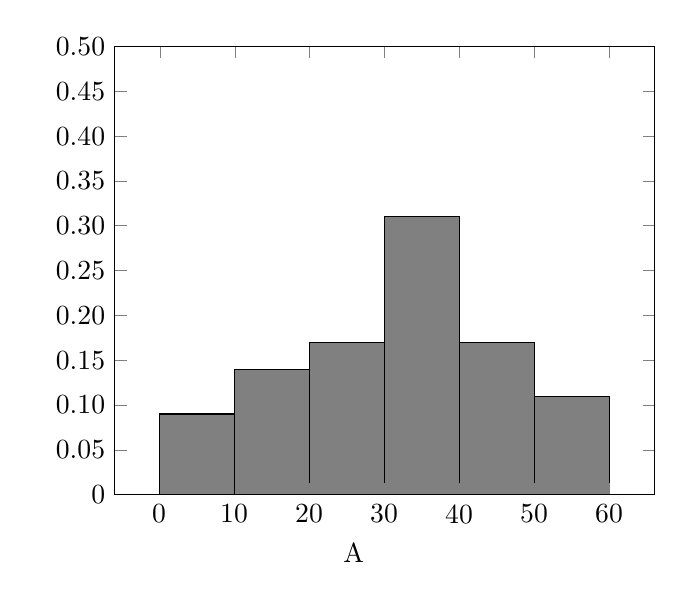
\begin{tikzpicture}
\begin{axis}[ytick={0, 0.05, 0.10, 0.15, 0.20, 0.25, 0.30, 0.35, 0.40, 0.45, 0.50},yticklabels={0, 0.05, 0.10, 0.15, 0.20, 0.25, 0.30, 0.35, 0.40, 0.45, 0.50}, ymax=0.50,ymin=0, area style, xlabel={A中学校の通学時間}, ylabel={相対度数}]
\addplot+[ybar interval, mark=no, fill = {gray}, draw = {black}] plot coordinates { (0, 0.09) (10, 0.14) (20, 0.17) (30, 0.31) (40, 0.17) (50, 0.11) (60, 0.00) };
\end{axis}
\end{tikzpicture}

\columnbreak

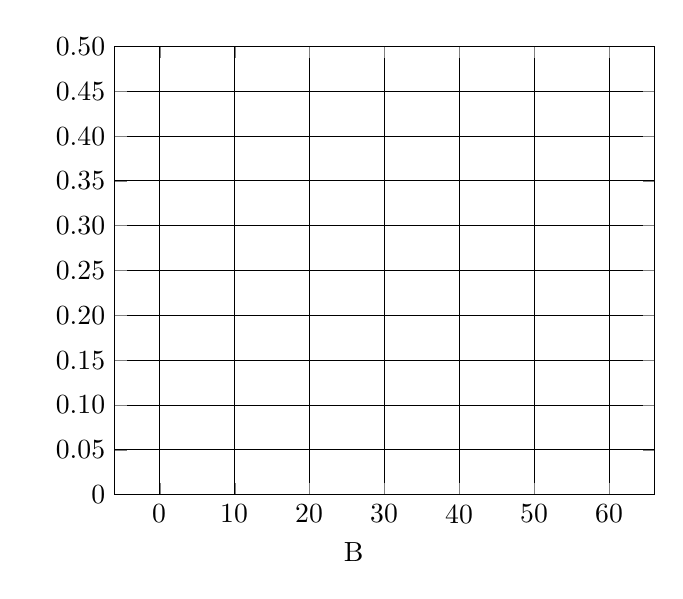
\begin{tikzpicture}
\begin{axis}[ytick={0, 0.05, 0.10, 0.15, 0.20, 0.25, 0.30, 0.35, 0.40, 0.45, 0.50},yticklabels={0, 0.05, 0.10, 0.15, 0.20, 0.25, 0.30, 0.35, 0.40, 0.45, 0.50}, ymax=0.50,ymin=0, area style, xlabel={B中学校の通学時間}, ylabel={相対度数}, grid = both, grid style = {black}]
\addplot+[ybar interval, mark=no] plot coordinates { (0, 0) (10, 0) (20, 0) (30, 0) (40, 0) (50, 0) (60, 0) };
\end{axis}
\end{tikzpicture}

\end{multicols}

\begin{center}
\textbf{※ 問題は次のページに続きます。}
\end{center}

\vfill

\newpage

(\text{\refstepcounter{skaunta}%
\arabic{skaunta}})\hspace{2.5pt}A中学校とB中学校において、どちらのほうが通学時間が長い傾向にあるかを\textbf{割合}という言葉を使って説明しなさい。ただし、通学時間が長いとは、通学に40分以上かかることとします。

\vspace{20mm}

(\text{\refstepcounter{skaunta}%
\arabic{skaunta}})\hspace{2.5pt}B中学校で一人に声をかけて通学時間が40分未満である確率は、どのくらいだと考えられますか。

\vspace{50mm}

\begin{multicols*}{2}

\noindent\fbox{\large\makebox[1em]{\text{\refstepcounter{kaunta}%
\arabic{kaunta}}}} \hspace{1pt}右の図形を、直線$l$を回転の軸として1回転させてできる立体の体積を求めなさい。

%
\begin{flushright}%
\footnotesize{<思・判・表3点>}%
\end{flushright}%


\vfill\null

\columnbreak

\begin{center}
\def\@captype{figure}
\includegraphics[height=35mm]{img/img15.jpg}

\end{center}

\end{multicols*}


\end{flushleft}

\end{document}
